\chapter{基于时空Transformer的运动重定向方法}
本章将详细介绍本文提出的基于时空 Transformer 架构的人机运动重定向算法——TransRetarget。
该算法旨在解决现有重定向方法中存在的帧间动作不连贯、对输入噪声敏感以及跨平台适配困难等核心问题。
\section{PoseformerV1}
作为本论文算法的参考算法，本文将首先介绍 PoseFormerV1 的原理。其主要完成的任务是解析输入的二维关键点序列，并生成相应的三维姿态表示。
PoseFormerV1 的整体架构主要由空间 Transformer 编码器和时间 Transformer 编码器级联而成
\cite{zheng3dHumanPose2021}\cite{zhaoPoseformerv2ExploringFrequency2023}，如图\ref{fig:poseV1network} 所示。

\begin{figure}
    \centering
    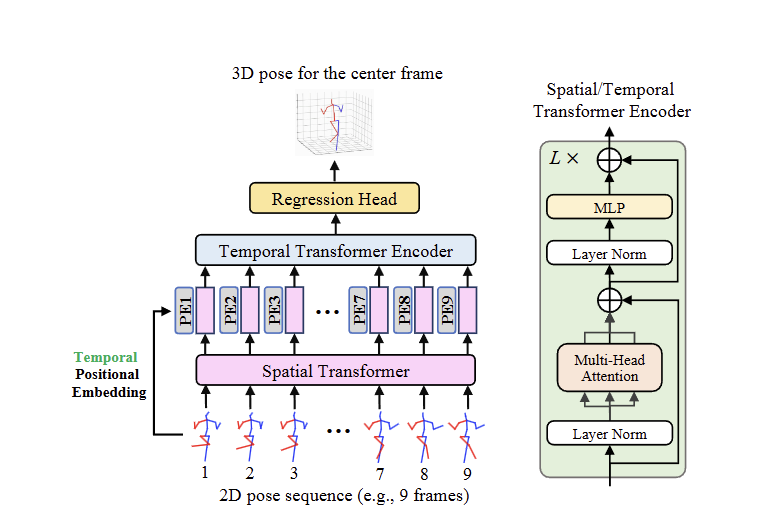
\includegraphics[width=0.9\textwidth]{figure/poseV1network.png}
    \caption{PoseFormerV1 的网络架构示意图。}
    \label{fig:poseV1network}
\end{figure}

\subsection{空间 Transformer 编码器}
输入：每一帧内所有人体关节的坐标 。

处理机制：首先将每个关节坐标线性投影为高维向量，并加入可学习的空间位置嵌入以保留关节类别信息，
然后将得到的向量输入至自注意力模块以生成空间特征，最后送至输出层以生成空间特征 。

作用：利用自注意力机制在单帧内捕捉不同关节之间的空间拓扑依赖关系 。
\subsection{时间 Transformer 编码器}
输入：将空间编码器输出的每一帧关节特征展平并拼接，转化为帧序列特征 。

处理机制：加入时间位置嵌入后，在整个时间维度上进行密集建模 。

作用：学习动作在长距离时间序列中的演变规律和动态特征 。
\subsection{回归头}
通过回归头聚合时间信息，并利用线性投影层最终输出中心帧的 3D 姿态表示 。
\subsection{主要优势}
打破卷积局限：相比传统的 CNN 方法，
PoseFormerV1 能够更好地建模人体关节间的长距离依赖和复杂的时间动态规律。
其在 Human3.6M 等权威数据集上取得了领先的预测精度，证明了 Transformer 处理骨骼点序列的有效性 。
\subsection{局限性}
尽管 PoseFormerV1 表现优异，但在实际应用中仍面临挑战。
其计算开销巨大：由于自注意力机制的计算量随序列长度成平方级增长，
处理长序列（如 81 帧以上）时对硬件资源要求极高。此时会导致计算时间增加，难以满足实时性要求。

\begin{figure}[t]
  \centering
  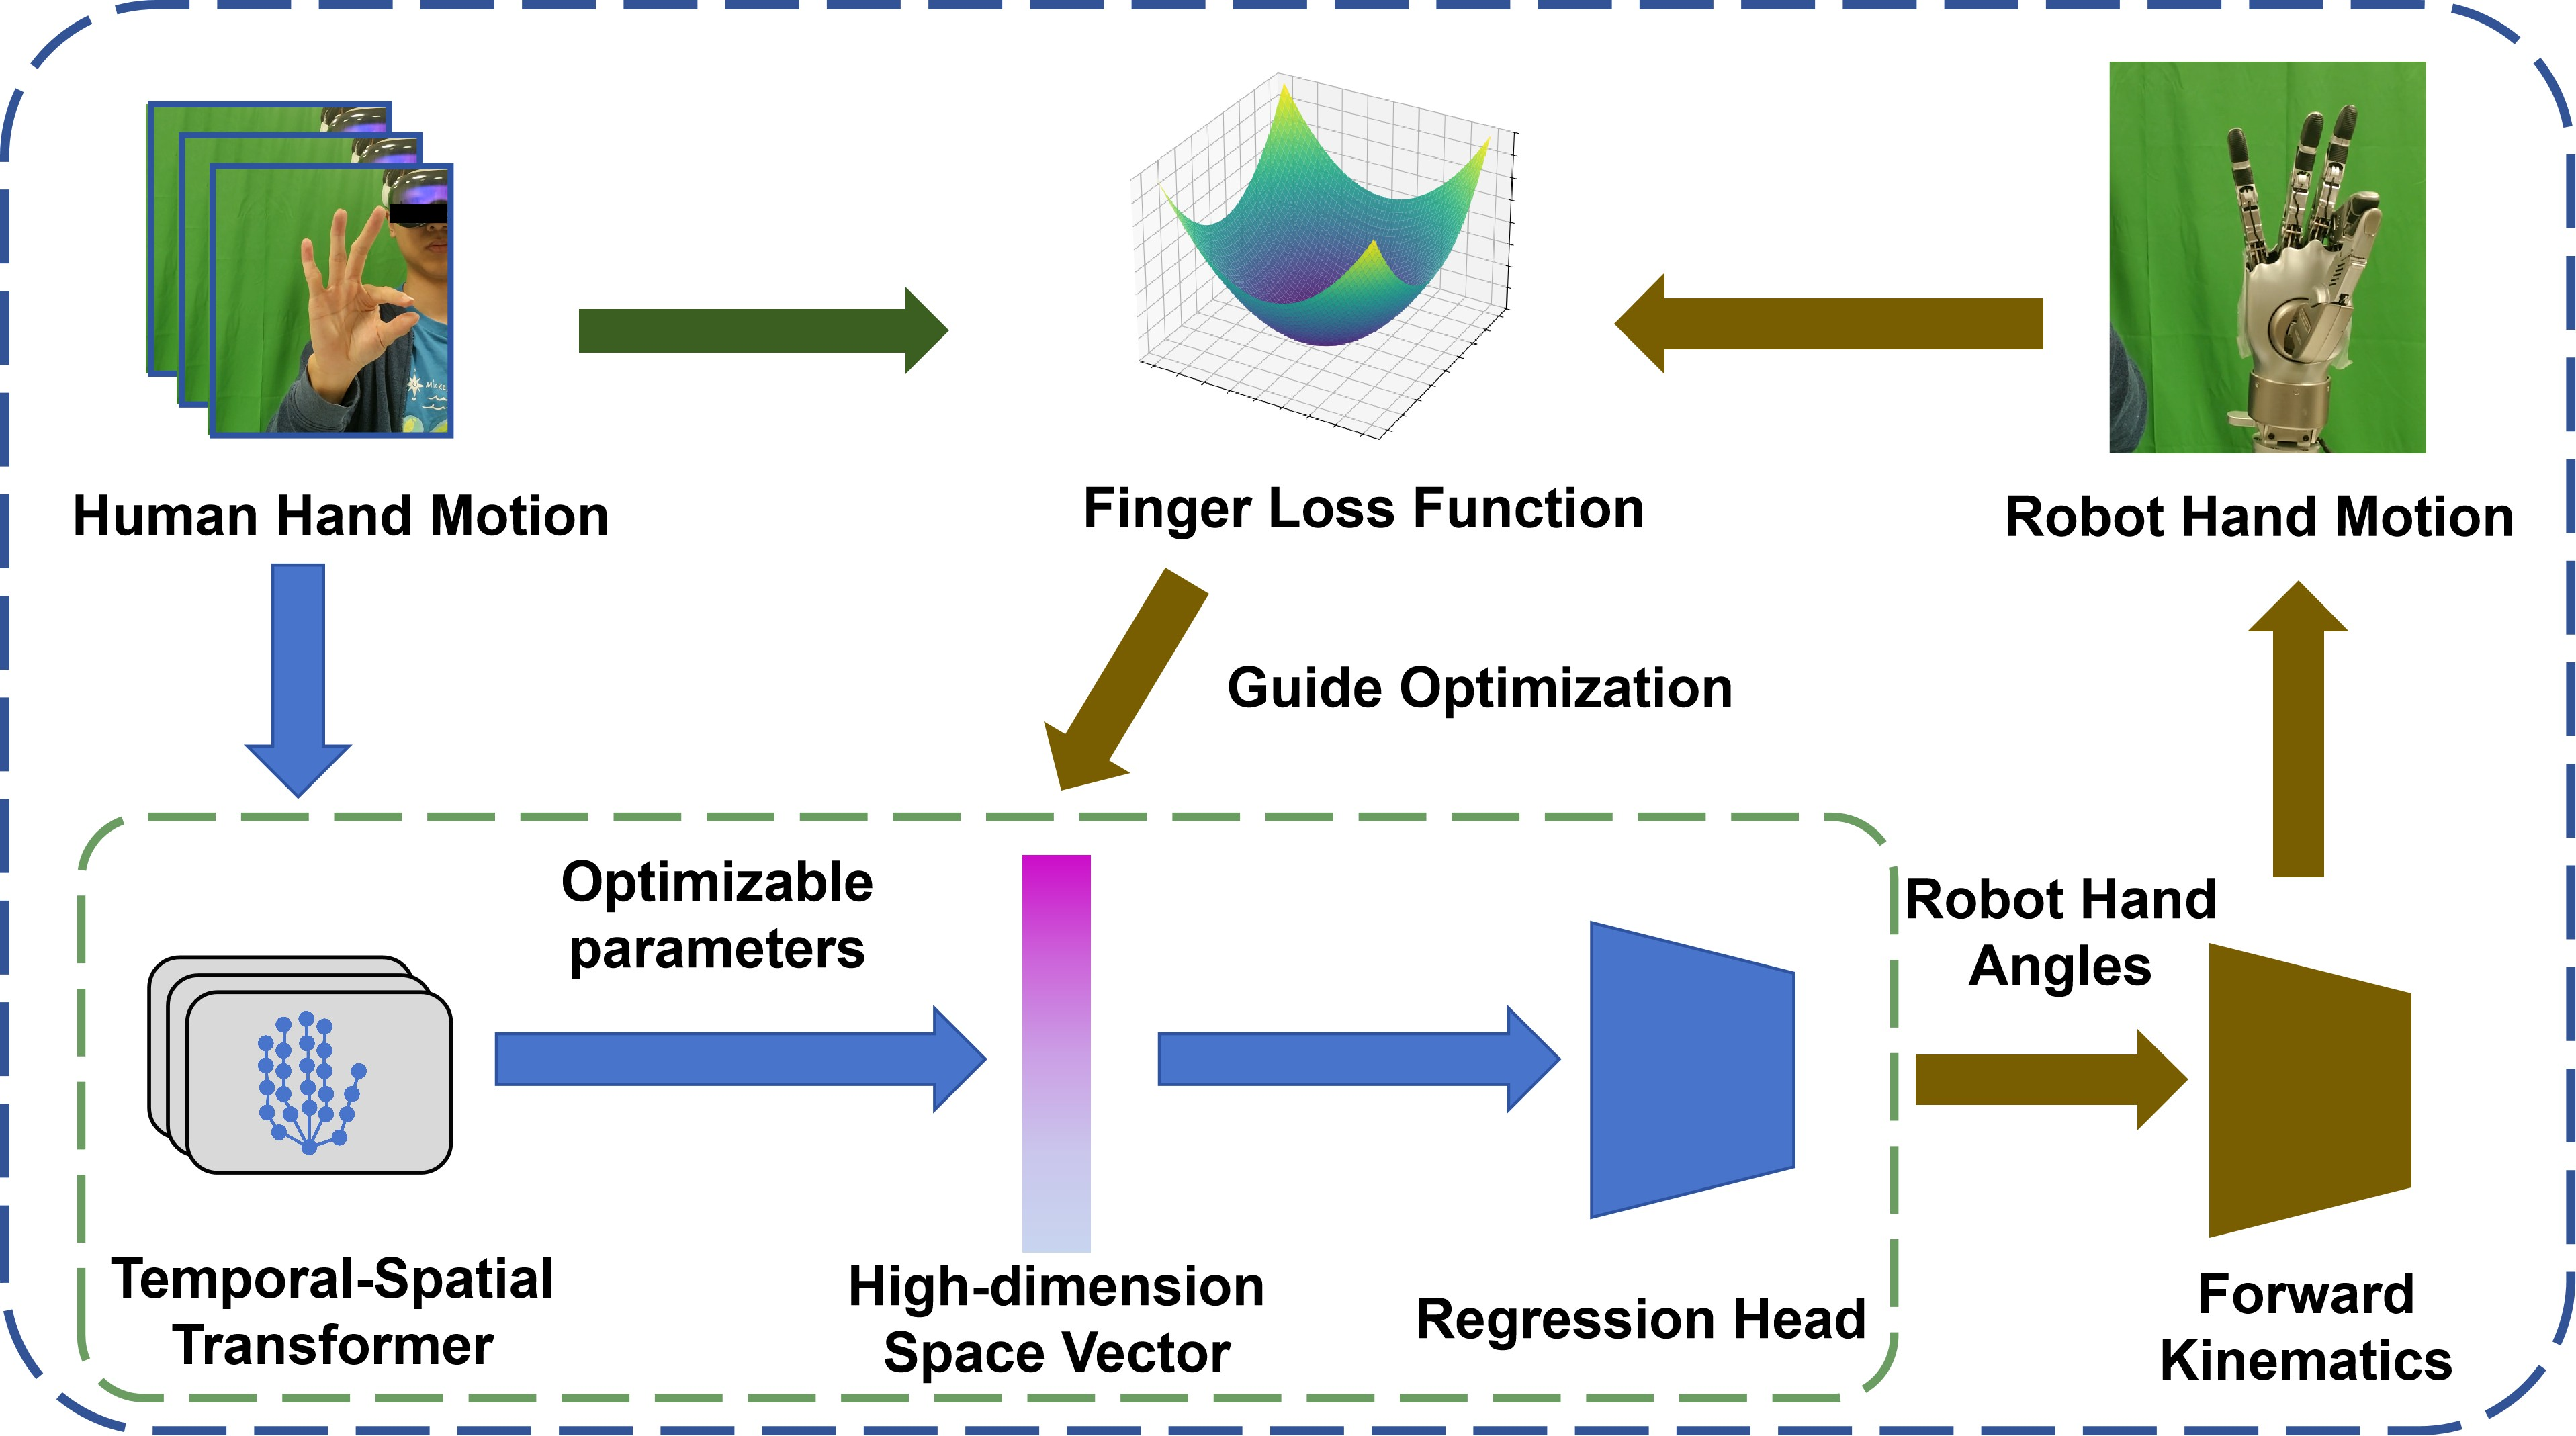
\includegraphics[width=0.95\textwidth]{figure/model_framework.jpg}
  \captionsetup{font=footnotesize}
  \caption{Overview of TransRetarget framework. The model input is the position of human joints. 
  During the training stage, after the angles are output, 
  they will be converted into the position of the robotic hand through the forward kinematics module, 
  and then enter the loss function to guide the optimization of network parameters, while the data flows along the blue arrows and the brown arrows. 
  In the inference process, the angles are directly used to drive the robotic hand, while the data flows along the blue arrows.
  }
  \label{fig:model_framework}
\end{figure}
\section{TransRetarget方法总览}
为了解决前述的问题，本文提出了 TransRetarget 方法，该方法通过引入时空 Transformer 架构，
实现了对人机手部运动的高效重定向。如图 \ref{fig:model_framework} 所示，
TransRetarget 的整体框架包括输入处理、时空特征提取、回归输出、运动学模块以及损失计算等关键模块。

在训练阶段，首先输入方面，我们将连续多帧数据统一坐标系，
输入到时空 Transformer 模块中，并生成包含时空特征的序列。然后我们将时空特征序列输入至回归头，
生成机器人手部关节角度。最后我们还会通过运动学模块将角度映射为机器人手部的实际位姿，并与人手的目标位姿进行对比，计算损失函数以指导网络优化。

而在实时推理阶段，我们输入实时的手部关节坐标，使用训练好的模型，使用固定的网络参数进行推理，从而实现人机手部运动的实时重定向。

\section{人手坐标系统一}
选择三个点构建平面构建坐标系，并选择两个点作为坐标轴，将两个点之间的向量作为坐标轴的法向量。

\begin{figure}[t]
  \centering
  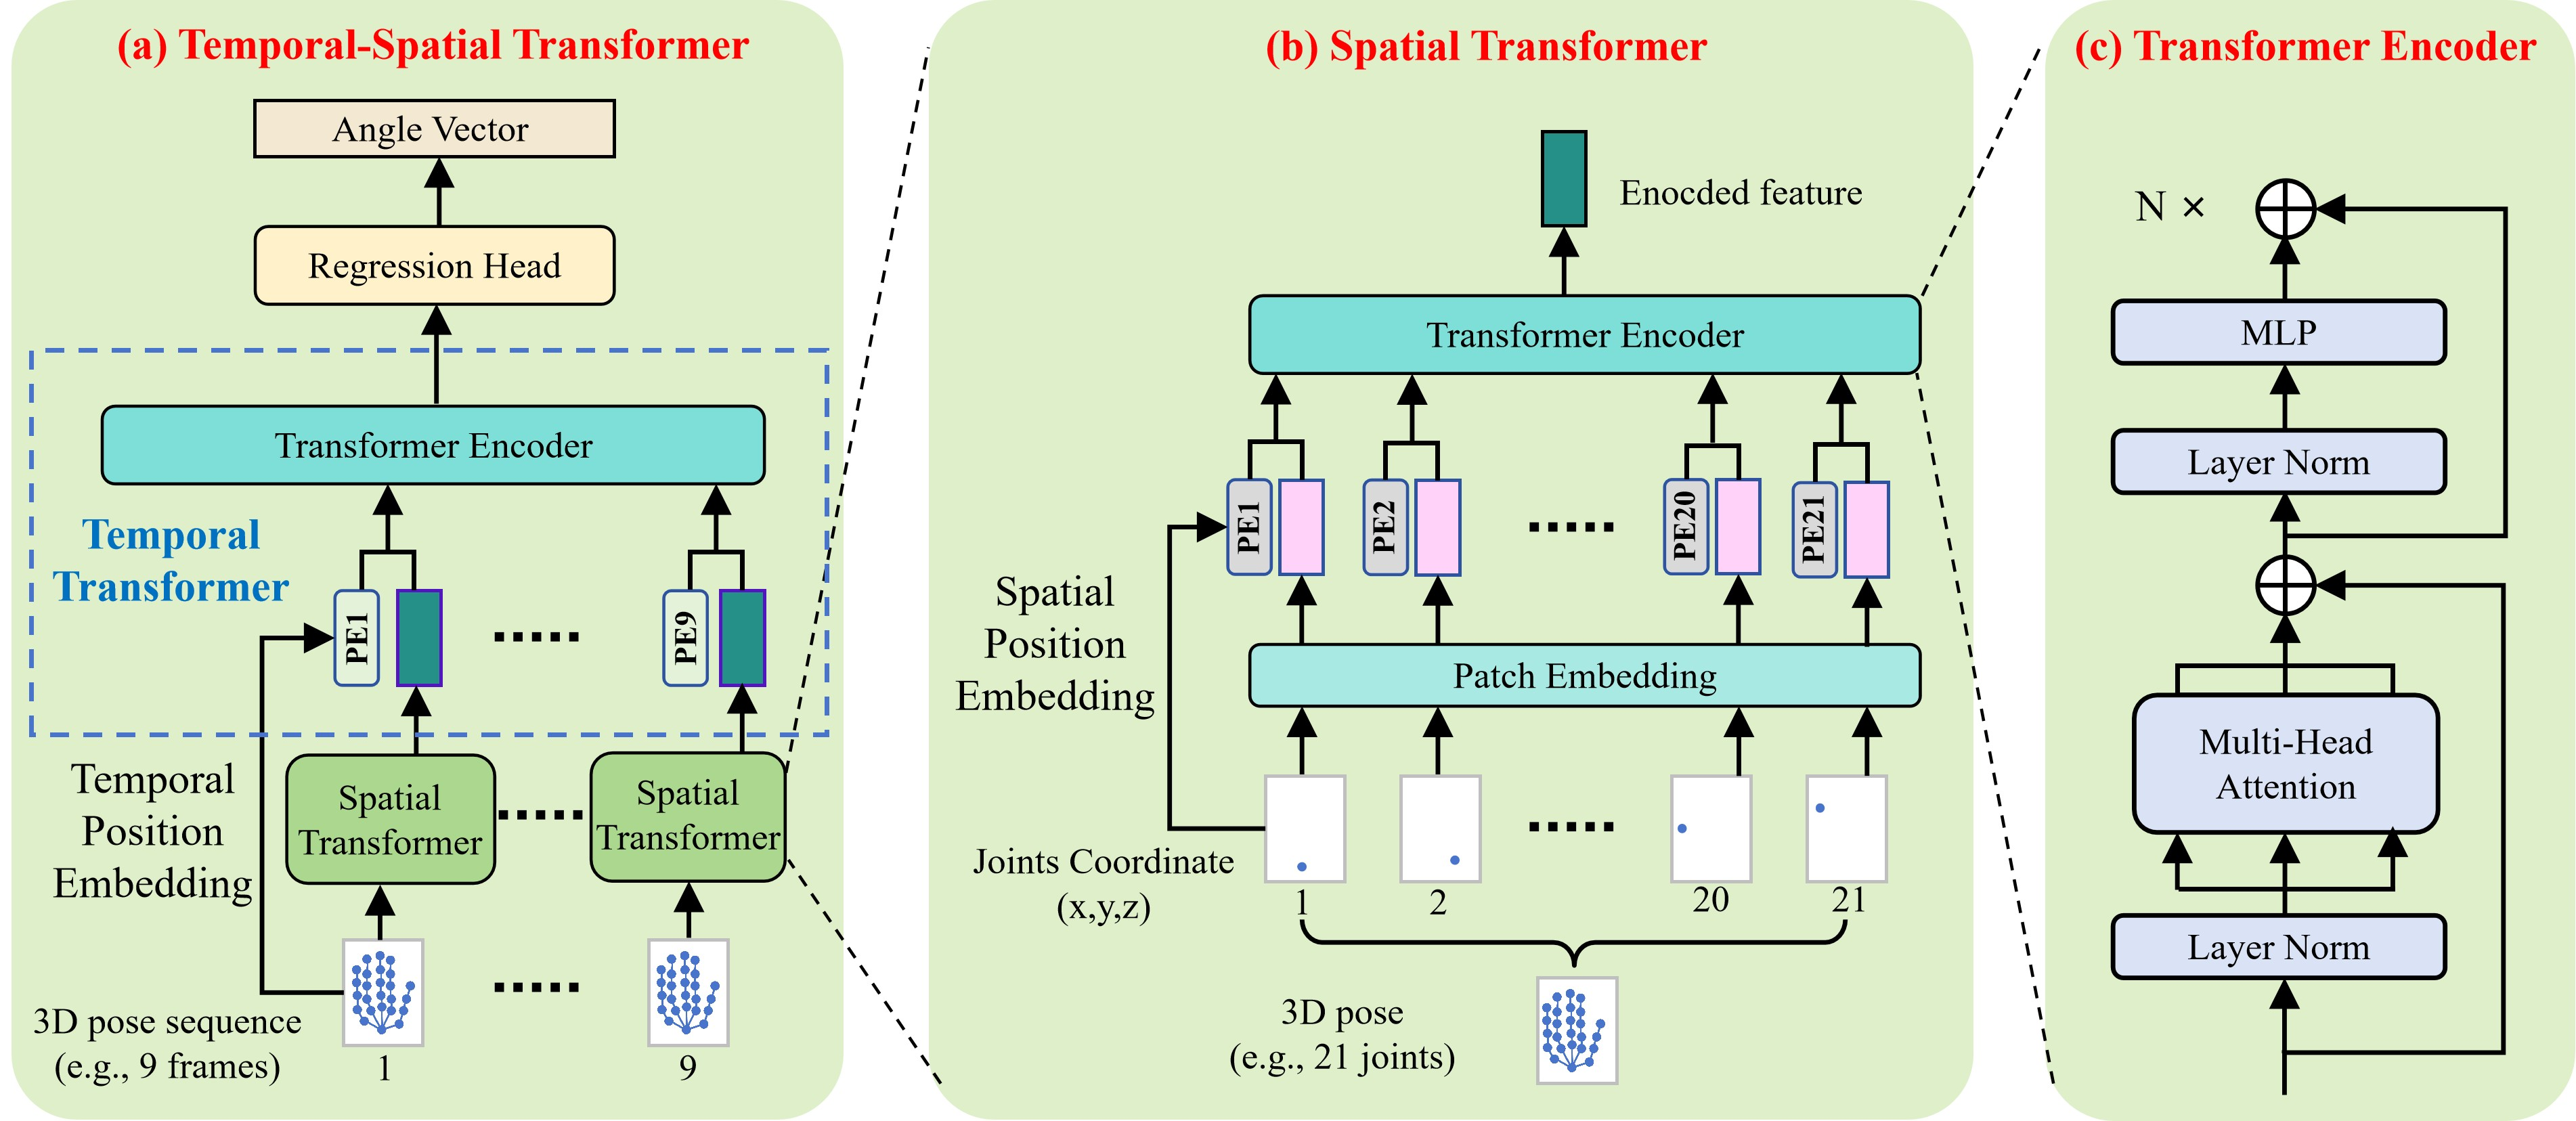
\includegraphics[width=0.95\textwidth]{figure/nextwork_framework.jpg}
  \captionsetup{font=footnotesize}
  \caption{ 时空Transformer模块的网络架构示意图。 
  输入为连续多帧手部关键点序列，经过空间编码器处理后，生成包含空间特征序列。然后输入至时间编码器，捕捉帧间信息，
  生成包含时空特征的序列。最后通过回归头将时空特征映射为机器人关节角度。
  (a) 时空Transformer模块; (b) 空间Transformer模块; (c) Transformer编码器.
  }
  \label{fig:network_framework}
\end{figure}
\section{空间编码器}
\label{sec1}
在本文提出的 TransRetarget 框架中，空间编码器承担着解析单帧手部姿态内部拓扑结构的任务。与原始 PoseFormerV1 处理 2D 像素坐标不同，
本文的空间编码器直接作用于三维空间数据，旨在提取更高维度的手部几何特征。
\subsection{特征线性投影}
空间编码器的输入为单帧手部关键点的三维坐标序列。为了使网络能够处理这些原始数值，
系统首先通过一个线性投影层将每个关键点的三维坐标映射到高维特征空间。
这一过程将离散的物理位置转化为具有丰富语义表达能力的特征向量，为后续的自注意力计算奠定基础。
\subsection{空间位置嵌入}
由于 Transformer 本身无法识别输入序列中不同关键点的物理属性，本文在特征向量中注入了可学习的空间位置嵌入。
这一设计确保了模型能够感知手部关节顺序，从而学习到符合人类生理结构的姿态信息。
空间编码器的核心是由多个多头自注意力模块组成的层级结构。在该模块中，每个关节特征都会与其他所有关节特征进行交互计算：
\subsection{空间多头自注意力机制}
模型会自动计算关节之间的关联权重，例如在执行抓取动作时，指尖与掌心关键点之间会分配更高的注意力权重。
通过层层深入的特征聚合，空间编码器能够提取出超越简单坐标关系的局部运动特征和整体手势语义。

\section{时间编码器}
\ref{sec1} 节提出的目标区域提取方法可以在均匀性或一致性的前提下将图像目标物体或目标区域分割出来,若与相邻部分合并则会破坏这种一致性。
时间编码器是 TransRetarget 框架中处理时序依赖性的核心模块。它的主要任务是接收空间编码器输出的特征序列，通过建模帧与帧之间的动态演变规律，提取手部运动在时间维度上的深层特征，从而确保重定向生成的动作序列具有物理平滑性。
\subsection{时间位置嵌入}
空间编码器将每一帧的手部空间拓扑结构转化为高维特征向量。时间编码器则将这些连续帧的特征向量重新排列，
形成一个具有时间属性的序列。为了使模型能够感知动作发生的先后顺序，本模块在输入端引入了时间位置嵌入。
这些位置信息与空间特征相融合，
使 Transformer 能够识别出动作的起始、延续与结束。
\subsection{时间多头自注意力机制}
时间编码器采用了多层自注意力机制来捕捉长距离的时间依赖关系。相比于逐帧处理的传统算法，该模块能够同时关注当前帧及其前后多帧的运动上下文：
通过计算不同时刻特征之间的注意力权重，模型能够学习到手指弯曲的速度、加速度等高阶运动属性。
在输入数据存在微小噪声或视觉遮挡导致关键点跳变时，
时间编码器可以利用邻近帧的运动惯性对当前时刻的特征进行修正，从而过滤掉非物理的高频抖动。
\subsection{时空特征深度耦合}
在该模块中，空间编码器提取的解剖学关联与时间编码器提取的运动趋势得到了深度耦合。这种设计使得模型不再仅仅关注单个静态姿态的还原，
而是从全局视角理解一段完整的动作语义。例如，在处理一个完整的抓取动作时，时间编码器能够确保指尖在闭合过程中的平滑过渡，
以及与手臂抬起动作的时序协同。由于引入了时间编码器，TransRetarget 克服了传统重定向方法中的抖动问题。
通过对多帧信息的整合，系统输出的关节控制指令不再是彼此孤立的点，而是符合动力学规律的连续曲线。这不仅提升了机器人运动的视觉自然度，
也有效减轻了物理电机的机械损耗，为实时遥操作提供了更加稳定的控制基准。

\section{回归头}
回归头是 TransRetarget 框架的输出层，负责将时间编码器提取的高维时空特征映射为机器人可执行的关节控制参数。该模块起到了连接深度神经网络特征与物理机器人运动学模型的桥梁作用。
\subsection{特征聚合与降维}
时间编码器输出的特征矩阵包含了多帧手部运动的复杂关联信息。回归头首先通过一个线性投影层或全连接层对这些特征进行空间维度的聚合，提取出与关节角度最为相关的语义分量。这一步骤有效地去除了冗余特征，将抽象的神经元激活值转化为具有明确物理意义的中间向量。
\subsection{关节角度向量映射}
在特征聚合的基础上，回归头利用非线性激活函数与线性映射的组合，将特征向量转换为目标机器人的关节角度向量。该向量的维度与目标灵巧手的自由度数量保持一致。例如，在 Linker 灵巧手平台上，回归头会输出一个 17 维的向量，每一维对应一个特定舵机或电机的目标旋转角度。
\subsection{物理范围限制与激活设计}
为了确保生成的角度向量初步符合硬件规范，回归头在输出层采用了 Sigmoid 或 Tanh 等激活函数，并配合比例缩放系数，将网络输出限制在机器人关节的物理极限范围内。这种预处理机制降低了后续运动学模块在处理越界数据时的计算压力。
\subsection{对后续运动学模块的支持}
回归头输出的关节角度向量是后续前向运动学模块的核心输入。通过将时间编码器捕捉到的平滑时序特征直接转化为角度，回归头确保了生成的指令流不仅在空间上能准确还原人手姿态，在时域上也能保持逻辑一致。这种端到端的映射方式极大地缩短了从视觉感知到动作控制的反馈链路，为实现高频率、低延迟的运动重定向提供了保障。
\section{运动学模块}
运动学模块是连接虚拟算法与物理实体的核心纽带，其主要功能是将回归头输出的关节角度映射为机器人在三维空间中的实际位姿。该模块通过解析标准机器人描述文件，构建出精确的几何变换链。

\subsection{机器人描述文件解析}
系统首先通过读取统一机器人描述格式（URDF）文件来获取目标机器手的物理参数。URDF 文件详细记录了机器人各连杆（Link）的几何尺寸、质量分布，以及各关节（Joint）的父子级层级关系。

位置偏移量：模块从文件中提取相邻关节间的相对平移参数，定义了机械结构的初始骨架。

旋转偏移量：通过读取关节轴线的方向和初始旋转偏置，确定了每个自由度的运动范围和旋转基准。

\subsection{前向运动学计算}
在获取固定结构参数后，运动学模块接收来自回归头的实时关节角度输入。利用前向运动学（FK）算法，系统沿运动链逐级进行齐次变换矩阵的连乘运算：

局部变换：根据当前输入的角度，计算每个关节相对于其父级关节的旋转矩阵。

全局映射：将所有局部的变换累积，最终推导出各关节相对于机器人手掌基座坐标系的精确三维位置。

\subsection{实际位置导出与物理校验}
该模块最终导出机器手各关键点在空间中的实际坐标。这些坐标不仅用于在仿真环境中实时同步机器人的姿态，还用于计算运动重定向的损失函数。
在导出位置的同时，模块会结合 URDF 中的物理限制，校验生成的姿态是否产生自碰撞或超出机械限位。

\subsection{跨平台适配的灵活性}
由于该模块完全基于 URDF 文件驱动，给予了TransRetarget 展现出的极强的平台适应性。当需要更换实验平台（如从 Linker 手迁移至 Shadow 手）时，仅需加载对应的配置文件，运动学模块即可自动更新所有变换参数，无需重新编写底层计算逻辑。
\section{损失函数设计}
为了引导 TransRetarget 框架学习到既符合物理逻辑又能精准还原人类意图的动作映射，本文设计了一套复合损失函数。该损失函数由四个核心部分组成，分别从局部关节配置、全局末端对齐、空间几何关系以及物理安全性维度对模型进行约束。

\subsection{手指摆动损失}
手指摆动损失主要用于约束机器人关节角度的合理性。该项通过对比人手关键点计算出的参考角度与回归头输出的机器人关节角度，确保每一根手指的运动趋势（如弯曲、伸展或侧向摆动）与人类保持语义一致。这有效防止了机器人关节出现非自然的扭转或违反生理结构的姿态。
\begin{equation}
L_{fv} = \frac{1}{N}\sum_{i=1}^{N} \left\| \frac{\mathbf{v}_{i}}{\|\mathbf{v}_{i}\|} - \frac{\hat{\mathbf{v}}_{i}}{\|\hat{\mathbf{v}}_{i}\|} \right\|^2.
\end{equation}
\subsection{手指指尖位置损失}
这是衡量重定向精度最直接的指标。该损失项计算经过前向运动学模块导出的机器人指尖三维坐标与经过缩放后的人手对应指尖坐标之间的欧式距离。通过最小化该距离，模型能够确保机器人在执行遥操作任务时，其末端执行器能够精准地到达目标空间位置，为后续的精细操作奠定基础。
\begin{equation}
L_{tv} = \frac{1}{N}\sum_{i=1}^{N} \left\| \frac{\mathbf{t}_{i}}{\|\mathbf{t}_{i}\|} - \frac{\hat{\mathbf{t}}_{i}}{\|\hat{\mathbf{t}}_{i}\|} \right\|^2.
\end{equation}

\subsection{手指指尖距离损失}
为了提高多指协作任务（如捏取、握持）的成功率，本文引入了指尖距离损失。该项不仅关注单个指尖的绝对位置，还关注不同指尖之间的相对空间距离。例如，当人手执行“对捏”动作时，该损失会强制机器人相应的手指指尖也保持较近的距离。这一设计补偿了单点定位误差带来的干涉或闭合不严问题，显著提升了抓取动作的鲁棒性。
\begin{equation}
L_{td} = \frac{1}{N}\sum_{i=1}^{N} \left\| \mathbf{d}_{i} - \hat{\mathbf{d}}_{i} \right\|^2.
\end{equation}
\subsection{碰撞损失}
碰撞损失是确保系统物理安全性的重要保障。该项基于运动学模块导出的各连杆空间位置，计算机器人自身各部件（如相邻手指之间）是否存在空间重叠。当检测到潜在的自碰撞风险时，该损失项会产生极大的惩罚值，引导模型调整关节角度以规避物理干涉。这不仅保护了昂贵的硬件设备免受损坏，也确保了生成的动作序列在现实世界中是可执行且安全的。
\begin{equation}
L_{col} = \sum_{c_{i,j} < c_{min}} -\log(c_{i,j}).
\end{equation}

\subsection{复合损失函数汇总}
最终的总体损失函数由上述四项加权累加而成。通过调整各部分的权重比例，模型能够平衡“位置精度”与“物理平滑性”之间的关系，最终输出一套既精准又平稳的控制指令流。
\begin{equation}
L_{total}=\lambda_{fv} \cdot L_{fv} + \lambda_{tv} \cdot L_{tv} + \lambda_{td} \cdot L_{td} + \lambda_{col} \cdot L_{col}.
\end{equation}
\section{本章小结}
本章阐述了图像局部颜色编辑方法中图像目标区域提取的相关方法，……
